\documentclass[12pt]{article}

\usepackage{amssymb,amsmath,amsfonts,eurosym,geometry,ulem,graphicx,caption,color,setspace,sectsty,comment,footmisc,caption,natbib,pdflscape,subfigure,array,hyperref}

\normalem

\onehalfspacing
\newtheorem{theorem}{Theorem}
\newtheorem{corollary}[theorem]{Corollary}
\newtheorem{proposition}{Proposition}
\newenvironment{proof}[1][Proof]{\noindent\textbf{#1.} }{\ \rule{0.5em}{0.5em}}

\newtheorem{hyp}{Hypothesis}
\newtheorem{subhyp}{Hypothesis}[hyp]
\renewcommand{\thesubhyp}{\thehyp\alph{subhyp}}

\newcommand{\red}[1]{{\color{red} #1}}
\newcommand{\blue}[1]{{\color{blue} #1}}

\newcolumntype{L}[1]{>{\raggedright\let\newline\\arraybackslash\hspace{0pt}}m{#1}}
\newcolumntype{C}[1]{>{\centering\let\newline\\arraybackslash\hspace{0pt}}m{#1}}
\newcolumntype{R}[1]{>{\raggedleft\let\newline\\arraybackslash\hspace{0pt}}m{#1}}


\geometry{left=1.2in,right=1.2in,top=1.0in,bottom=1.0in}

\begin{document}

\begin{titlepage}
\title{A review of High Dimensional Nonlinear Data Dimension Reduction Methods
\thanks{Electronic address: \texttt{jaguirre31@gatech.edu}; Corresponding author}}
\author{Jacob Aguirre, Ruirui Ma, Shrey Patel}
\date{\today}
\maketitle
\begin{abstract}
\noindent Massive, high-dimensional data sets are already appearing in a variety of sectors of modern research, posing new obstacles. These high-dimensional data sets can typically be modeled as point clouds in a $D-$dimensional space, such that it's concentrated near a $d-$dimensional manifold. Thus, we are able to visualize this data as a low-dimensional representation. The well-known curse of dimensionality in machine learning suggests that a huge amount of training data is necessary in order to obtain a given prediction accuracy. Unless additional assumptions are established, picture and signal recovery requires a significant number of observations to recover a high-dimensional vector. Owing to the fact there exist rich localized constants, global symmetry, repeated patterns, or redundant sampling, many real-world data sets show low-dimensional geometric structures. This study seeks to investigate these local structures on a variety of simulated and real data-sets, and discover which properties contribute to certain models performing well or under performing. As a result, we're attempting to investigate low-dimensional geometric patterns in data sets in order to extract features, forecast data, and recover signals.  \\
\vspace{0in}\\
\noindent\textbf{Keywords:} High-Dimensional Data, Machine Learning, Statistical Inference\\
\vspace{0in}\\
\noindent\textbf{JEL Codes:} C15, C44, C45\\

\bigskip
\end{abstract}
\setcounter{page}{0}
\thispagestyle{empty}
\end{titlepage}
\pagebreak \newpage




\doublespacing


\section{Background} \label{sec:introduction}

\hspace{5mm}The $21^{st}$ century presents new challenges in the realm of statistical inference and data mining. High dimensional data sets are arising more often, which contributes to challenges in attempting to understand and draw conclusions from such data. For the purposes of image and signal recovery, a large amount of technical expertise is needed in order to recover a high-dimensional vector we're interested in [1].

Machine learning can assist us in comprehending enormous amounts of data and making judgments based on that information. However, in order to do so, we must first figure out how to extract the data's information effectively (and efficiently). Often times, we can visualize these data sets on a lower dimensional manifold. Consider the classic example of images, text files, or even sound waves. These can be expressed as a vector $x\in\mathbb{R}^n$. Thus, each element in this vector would correspond to a pixel, word, or signal, respectively.

In this work, we will seek to focus on 4 different methods. These are Isomap, T-SNE, Diffusion Maps, and Local Linear Embedding [2]. Each presents it's own unique methodology, pros, and cons. Within this report, we will, of course, provide the necessary background and prerequisite knowledge needed to understand each method. We will make sure to focus specifically on the applications, how well our methods worked, and the limitations with each. 

The rest of this paper is as follows: Section 2 introduces background of existing literature of nonlinear dimension reduction methods; Section 3 is split into 4 subsections, each discussing a different algorithm and the corresponding methodology. Section 4 provides a commentary of the results, as well as supplying an analytic approach to decide whether our hypothesis was correct for nonlinear dimension reduction methods; Section 5 presents concluding remarks and avenues of future research. Attached is an appendix, which will have all the graphs, charts, and tables we created.


\section{Literature Review}
\hspace{5mm}
The underlying neighbor-graph construction technique is common to many dimension reduction techniques.
Several non-linear dimension reduction techniques make the same initial assumption: suppose $X =\{x_1,..., x_n\}$ is a set of points lying on a manifold $\mathcal{M}$ embedded in ambient $\mathbb{R}^D$space. This manifold $\mathcal{M}$ is of a lower-dimension than $\mathbb{R}^D$, but it is not observed; only samples from this manifold are available (the observed X). From this discrete subset $X$, we seek to recover the manifold structure of $\mathcal{M}$.




\section{Local Linear Embedding} \label{sec:Local Linear Embedding}

\subsection{Motivation}
\hspace{5mm}
The beauty of the Local Linear Embedding algorithm lies in it's simple, geometric intuitions. This allows for both ease of understanding and implementation of the algorithm on real world data projects. Below, we seek to summarize how this algorithm works.

\begin{enumerate}
    \item Procedure of Algorithm
    \begin{itemize}
        \item First, we need to find the K-Nearest Neighbors. The advantage of KNN is that we only have one free parameter in the entire algorithm, $k.$
        \item We then perform a weighted aggregation of the neighbors for each point, to construct a new point. We seek to minimize the cost function presented below.
        \begin{equation}
            E(W)=\sum\limits_i|X_i-\sum\limits_jW_{ij}|^2 s.t. \sum\limits_jW_{ij}=1
        \end{equation}
        \item Now, we need to define a vector space $Y$ s.t. we minimize a new cost for Y with the new points.
        \begin{equation}
            C(Y)=\sum\limits_i|Y_i-\sum\limits_jW_{ij}Y_j|^2
        \end{equation}
    \end{itemize}
\end{enumerate}

\subsection{Approach}

\subsection{Results}

\section{Diffusion Map} \label{sec: Diffusion Map}

\subsection{Motivation}
Diffusion map is a computationally inexpensive non-linear dimensionality reduction technique that seeks to discover lower-dimensional structure embedded in high-dimensional data space. It finds a diffusion map that maps points in high dimensional data space onto lower dimensional diffusion space so that finding the euclidean distance in the diffusion space is equivalent in finding the diffusion distance in data space, which effectively mitigates the curse of dimensionality.
\subsection{Approach}
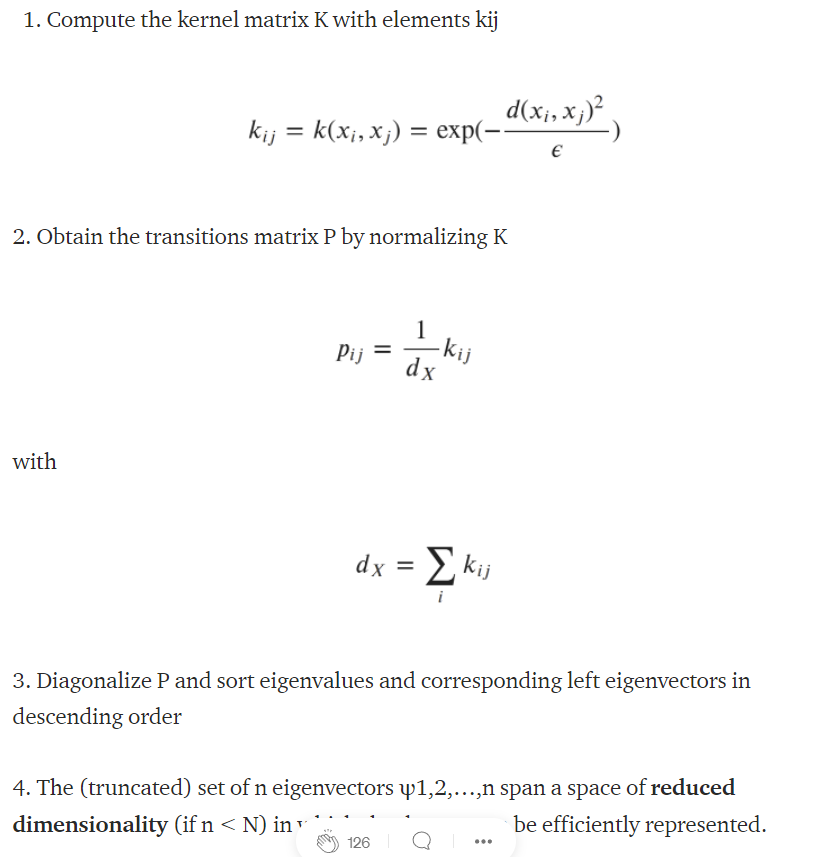
\includegraphics[scale=0.5]{algo.png}
\subsection{Results}

\section{T-SNE} \label{sec: T-SNE}
\subsection{Motivation}
\hspace{5mm}t-Distributed Stochastic Neighbor Embedding (t-SNE) forms a lower dimensional embedding using probability distributions to compute similarities between points across different dimensional spaces. By using a Student t-distribution to model the probabilities of points in the low dimensional space (LDS), t-SNE resolves the issue of SNE, which misrepresents dissmilar points in the high dimensional space (HDS) as close or related points in the LDS.

\subsection{Approach}
\hspace{5mm}While I used the "TSNE" function provided by the Python "sklearn.manifold" library, I will describe the t-SNE algorithm below.

\subsection{Results}

\section{Isomap} \label{sec: Isomap}


\subsection{Motivation}

\hspace{5mm}Isometric Feature Mapping (or ISOMAP) was first proposed by Tenenbaum, de Silva, and Langfor, and assumes that the data is near a smooth manifold. If the assumption is sound, concepts like neighborhood and local linearity can be used to map the manifold to a linear structure before reducing it with the help of a linear algorithm. Consider that oftentimes, a nonlinear dataset might be folded or curved, such is the often the shape of a manifold [5]. 


\subsection{Approach}
\hspace{5mm}For my review of the Isomap approach, let $\textbf{S}$ be the simulated data in the shape of a Swiss roll. A picture of the data is presented below and in the supplementary materials. Full code can be found hosted on github.

\begin{figure}[h!]
\centering    
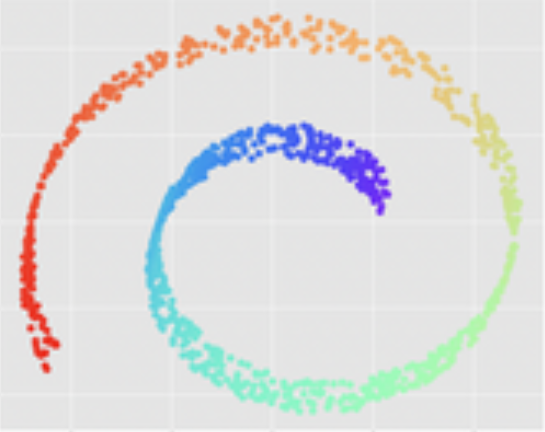
\includegraphics[width=100mm]{swissroll1.png}
\caption{Swiss Roll, N=1000, features=3}
\label{fig: Swiss Roll}
\end{figure}

\subsubsection{Construction of Algorithm}

\hspace{5mm}The basis of the algorithm can be described in 3 main points. Consider a dataset $\textbf{S}$ and let $p\in\mathbb{R}^n$ be the number of features we want to include in the reduced data [5].

\begin{enumerate}
    \item Procedure of Algorithm
    \begin{itemize}
        \item Construct a weighted graph \textbf{G} from the distances pairwise to some \newline$\delta_{xy},\forall (\textbf{x},\textbf{y})\in \textbf{X} \times \textbf{X},\textbf{x}\neq\textbf{y}.$ Next, we need to find the graph $G^{''}$ by applying a nearest neighbor algorithm on the graph $G$.
        \item Compute a shortest path graph $G^{''}$ between all pairs of nodes from the graph $G^'$.\newline For this computation, we make use of Dijkstra’s algorithm.
        \item Lastly, use $G^{''}$ to construct the $p$-dimensional embedding by using the Multidimensional scaling algorithm.
    \end{itemize}
\end{enumerate}

\hspace{5mm}

\subsection{Results}


\hspace{5mm}The Isomap Method worked quite efficiently on the Swiss roll dataset. The swiss roll contained around 1000 points, and so this made me hesitant on how well Isomap would perform. However, it does a pretty decent job of preserving the global structure of the original data.

\begin{figure}[h!]
    \centering
    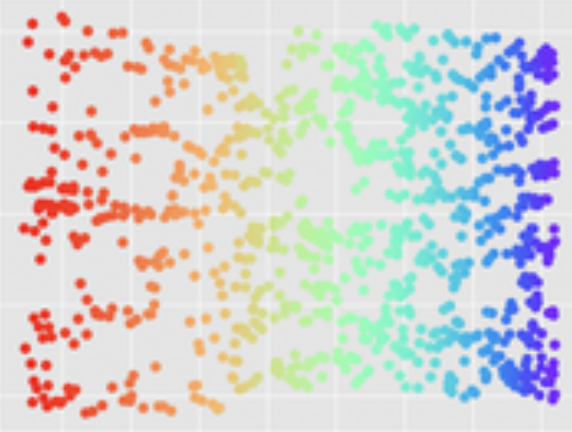
\includegraphics[width=100mm]{swissrollunrolled.png}
    \caption{Swiss Roll unrolled}
    \label{fig:swissunrolled}
\end{figure}


\newpage

\section{Discussion} \label{sec:discussion}

\hspace{5mm}


\subsection{Limitations}
\hspace{5mm}For this brief report, we sought to discuss the topic of nonlinear dimensionality reduction. First, we effectively reduced, displayed, and learnt from well-known data sets by focusing on linear algorithms and their ability to extract features that optimize variance in a data set. In addition, we illustrated how these techniques would not be able to decrease data sets with a nonlinear distribution.

Thus, this caused for us to seek out nonlinear dimension reduction techniques. For this, we utilized the following: T-SNE, Isomap, Diffusion Maps, and Local Linear Embedding (LLE). We found that each method had their merits and difficulties. For example, the isomap represents a step forward in manifold learning and was a widely used dimensionality reduction method until recently. Currently, Uniform Manifold Approximation and Projection (UMAP) had begun to take over the literature. In practice, its relevance can be seen in the large number of machine learning libraries, languages, and computational environments that use it, as well as the large amount of research done by numerous authors attempting to apply, improve, or expand it.

We end by concluding that this study was overall quite successful. We showed a multitude of different techniques, how well they will perform or fail on given data sets, and what to consider when using them. It's always important to note that within the realm of data science and statistical inference, a "one method fits all" approach is likely to fail. You must always be aware of the particularities within your dataset, and constantly tryout new methods to explore and find causal inference within. Thus, we kept this in mind when we performed all of our approaches and simulations.

\subsection{Future work}
\hspace{5mm}This project has taught us a great deal about the nature of nonlinear dimension reduction methods. This report has inspired us to continue further work in this area, and encouraged us to read journal papers related to the area. In doing so, we stumbled upon the evergrowing popular method, "Uniform Manifold Approximation and Projection" (UMAP) algorithm proposed again by Tenenbaum [12].

This algorithm can be considered seriously competitive with t-SNE for it's amazing visualization quality, and can actually manipulate the global structure more accurately. Below is a figure from a recent article written by a group of scientists from Johns Hopkins University [13]. As you can see, the data is formatted perfectly, and is much cleaner than t-SNE. 

\begin{figure}[h!]
\centering    
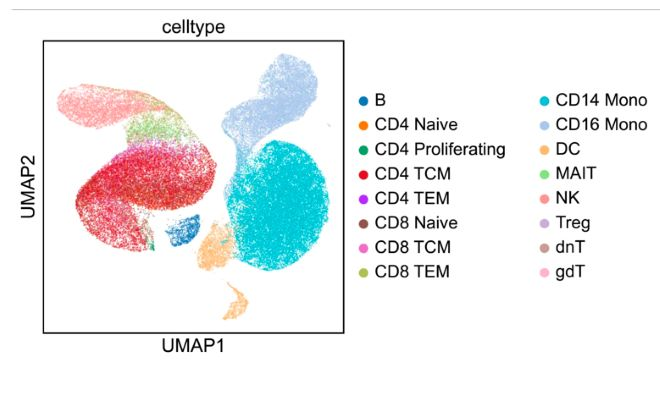
\includegraphics[width=100mm]{umap pic.jpg}
\caption{UMAP on cellular data}
\label{fig: UMAP}
\end{figure}





\newpage
\begin{thebibliography}{}
\bibitem{First Entry}Fannjiang, Albert, and Wenjing Liao. "Coherence pattern–guided compressive sensing with unresolved grids." SIAM Journal on Imaging Sciences 5.1 (2012): 179-202.

\bibitem{scikit learn}scikit learn, “Svm: Maximum margin separating hyperplane.” [Online].Available: http://scikit-learn.org/stable/auto$_$examples/svm/plot$_$separating$_$hyperplane.html.


\bibitem{UCI machine learning}M. Lichman, “UCI machine learning repository,” 2013

\bibitem{bioinformatics}P. Baldi and S. Brunak, Bioinformatics: The Machine Learning Approach. A
Bradford book, A Bradford Book, 2001.

\bibitem{geometric structure}J. Wang, Geometric Structure of High-Dimensional Data and Dimensionality
Reduction. Springer Berlin Heidelberg, 2012.

\bibitem{definitions}S. S. A. H. Renear and K. M. Wickett, “Definitions of dataset in the scientific
and technical literature,” ASIS&T 2010, 2010

\bibitem{algorithms for manifolds}L. Cayton, “Algorithms for manifold learning,” Univ. of California at San
Diego Tech. Rep, pp. 1–17, 2005.

\bibitem{MDS}T. Cox and M. A. A. Cox, Multidimensional scaling. Boca Raton, FL, USA:
CRC Press, 2000.

\bibitem{graph theory}W. Mayeda, Graph Theory. John Wiley & Sons, 1972.

\bibitem{elements of machine}P. Langley, Elements of Machine Learning. Machine Learning Series, Morgan
Kaufmann, 1996.

\bibitem{semi-supervised learning}X. Zhu and A. B. Goldberg, “Introduction to semi-supervised learning,” Synthesis lectures on artificial intelligence and machine learning, vol. 3, no. 1,
pp. 1–130, 2009

\bibitem{UMAP}McInnes, Leland, John Healy, and James Melville. "Umap: Uniform manifold approximation and projection for dimension reduction." arXiv preprint arXiv:1802.03426 (2018).

\bibitem{umap JHU}shorturl.at/clIQS

\bibitem{t-SNE}Laurens van der Maaten, and Geoffrey Hinton. “Visualizing Data Using T-SNE.” Journal of Machine Learning Research, vol. 1, 2008, pp. 1–48, www.cs.toronto.edu/$\sim\text{hinton/absps/tsne.pdf.}$



\end{thebibliography}


\section{Supplementary materials}

Try and put your tables, charts, images here! Simply cite them up top when you're writing your sections. Thanks :D

\section{Contributions}

\hspace{5mm}All three of us contributed to the writing of the introduction and literature review of this report. Shrey wrote the t-SNE section, Ruirui the Diffusion map, and Jacob wrote the Local Linear embedding, Isomap, and discussion sections. 

\end{document}